\begin{figure}[t!]
    \centering

    \captionof{table}{An inter-request contention example.}
    \label{tab:InterReqExample}

    \fontsize{9}{11}\selectfont
    \begin{tabular}{c|c|c|c|c}
        \toprule
        \textbf{Req ID} & \textbf{Flow ID} & \textbf{Flow Size} & \textbf{Remain time} & \textbf{Deadline} \\
        \midrule
        1   & A & 2 & 9 & 18 \\
        2,3 & B & 4 & 6 & 12 \\
        4   & C & 3 & 0 & 7  \\
        \bottomrule
    \end{tabular}

    \begin{subfigure}{0.48\columnwidth}
        \centering
        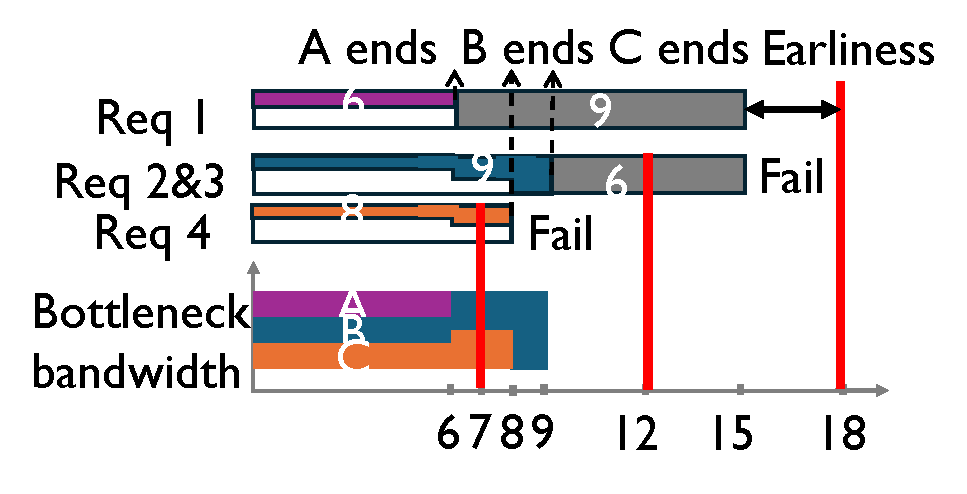
\includegraphics[width=\linewidth]{figures/methodology/InterContentionExample-FS.pdf}
        \caption{Fair Share}
        \label{fig:bg:expfs}
    \end{subfigure}
    \hfill
    \begin{subfigure}{0.48\columnwidth}
        \centering
        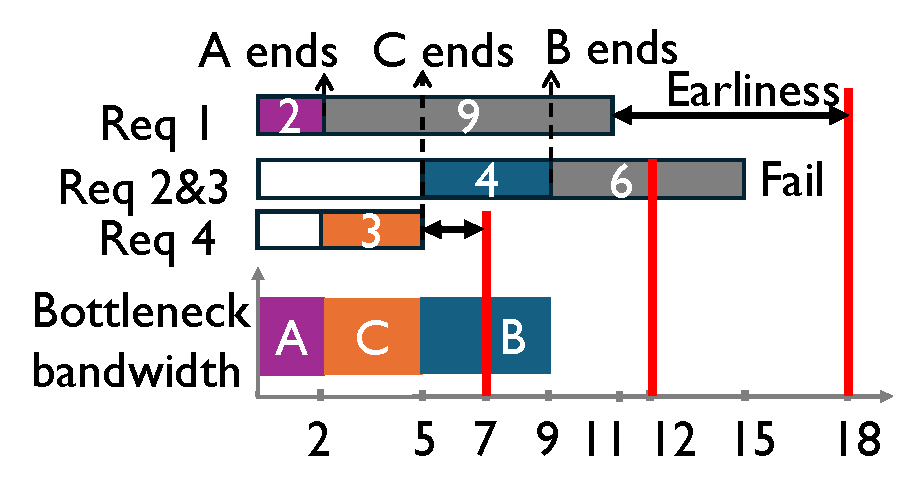
\includegraphics[width=\linewidth]{figures/methodology/InterContentionExample-SJF.pdf}
        \caption{Shortest Job First}
        \label{fig:bg:expsjf}
    \end{subfigure}

    \par\medskip

    \begin{subfigure}{0.48\columnwidth}
        \centering
        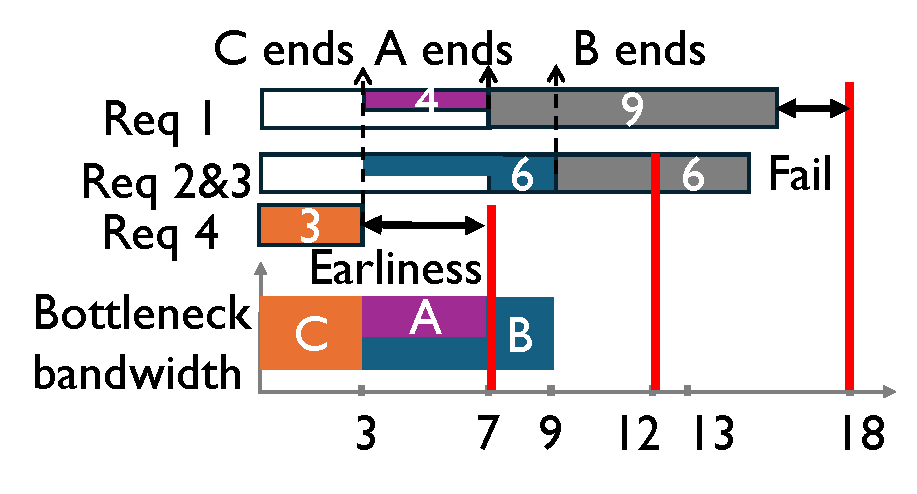
\includegraphics[width=\linewidth]{figures/methodology/InterContentionExample-EDF.pdf}
        \caption{Earliest Deadline First}
        \label{fig:bg:expedf}
    \end{subfigure}
    \hfill
    \begin{subfigure}{0.48\columnwidth}
        \centering
        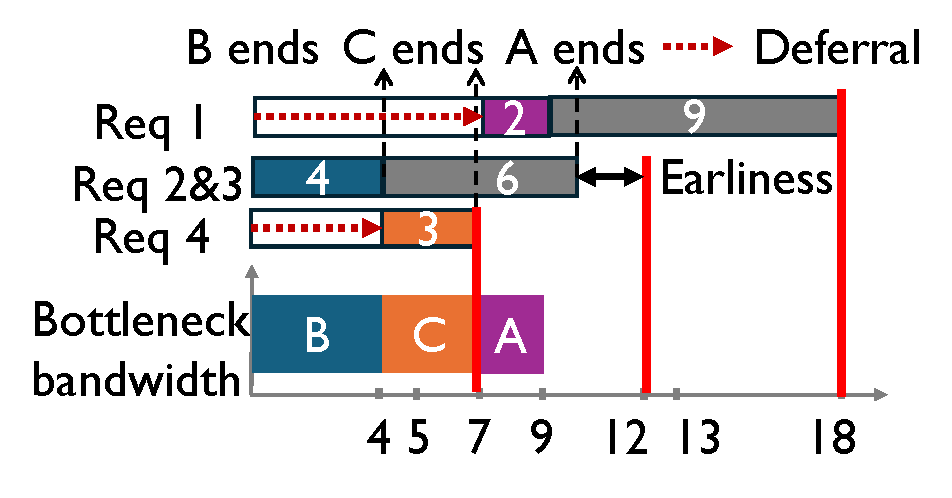
\includegraphics[width=\linewidth]{figures/methodology/InterContentionExample-DAP.pdf}
        \caption{Defer-and-Promote}
        \label{fig:bg:expopt}
    \end{subfigure}

    \caption{\textbf{Comparison of scheduling policies for inter-request contention.}
    The red vertical lines denote hard deadlines, and gray bars are subsequent durations.
    (a) Fair Share and (b) SJF fail to protect the urgent Flow-B due to lack of deadline awareness,
    while (c) EDF completes flows with explicit but loose deadlines unnecessarily early.
    (d) \DAP strategically defers non-urgent flows to minimize earliness,
    and promotes them only when necessary to achieve \textit{just-in-time completion}.}
    \label{fig:meth:inter}

    \vspace{-2em}
\end{figure}
